\chapter{Tecniche risolutive}
\label{capitolo:preliminari:ulteriori}


% In questo capitolo si introducono le premesse teoriche necessarie per la comprensione dei capitoli successivi.
% Oltre alle tecniche riscontrate durante l'analisi della letteratura si \`e scelto di introdurre altri concetti utili per ulteriori metodi risolutivi.

Questo capitolo introduce le premesse teoriche necessarie per la comprensione di: 
\begin{itemize}
  \item 
    Algoritmi usati nello stato dell'arte.
  \item
    Algoritmi usati nel sistema implementato.
  \item
    Algoritmi dei quali \`e stata valutata l'adeguatezza alla soluzione del problema.
\end{itemize}

L'organizzazione dei contenuti in sezioni \`e illustrata nella figura \ref{prerequSect}
% Oltre alla presentazione degli algoritmi descritti nell'analisi della letteratura si \`e dato uno spazio alla descrizione di algoritmi utili per la soluzione del problema.
% Dopo un analisi delle possibili tecniche risolutive si \`e scelto di suggerire un sistema che utilizza un algoritmo di onset detection insieme a un algoritmo di clustering. 




\begin{center}
\begin{figure}
 

\begin{tikzpicture}
%   [scale=.8,auto=left,every node/.style={fill=blue!20}]
[->,>=stealth',shorten >=1pt,auto,node distance=3cm,
  thick,main node/.style={circle,fill=blue!20,draw,font=\sffamily\Large\bfseries}]
  \node (n1) at (0,3) {tecniche};

  \node (n1n1) at (4,1) {stato dell'arte};
  \node (n1n2) at (4,3) {sistema implementato};
  \node (n1n3) at (4,5) {altre valutate};

%   \node (N1) at (8,2) {filtri};
  \node (N2) at (8,3) {onset detection};
  \node (n1n1n2) at (8,2) {modelli markoviani};
  \node (n1n1n3) at (8,1) {dimensione frattale};
  \node (n1n3n1) at (8,4) {clustering};
  \node (n1n3n2) at (8,5) {reti neurali};

  \node (N1n1) at (12,3) {\ref{beatdetectionDescrizione}};
%   \node (N1n2) at (12,3) {\ref{filtri}};
  \node (n1n1n2n1) at (12,2) {\ref{markov}};
  \node (n1n1n3n1) at (12,1) {\ref{frattale}};
  \node (n1n3n1n1) at (12,4) {\ref{clustering}};
  \node (n1n3n2n1) at (12,5) {\ref{retineurali}};

   \foreach \from/\to in {n1/n1n1,n1/n1n2,n1/n1n3,n1n1/N2,n1n2/N2,n1n2/n1n3n1,n1n1/n1n1n2,n1n1/n1n1n3,n1n3/n1n3n1,n1n3/n1n3n2, N2/N1n1,n1n1n2/n1n1n2n1,n1n1n3/n1n1n3n1,n1n3n1/n1n3n1n1,n1n3n2/n1n3n2n1}
     \draw (\from) -- (\to);

\end{tikzpicture}
\caption{Organizzazione dei contenuti nelle sezioni del capitolo}
\label{prerequSect}
\end{figure}
\end{center}




\section{Beat detection}
\label{beatdetectionDescrizione}
% Con il termine beat detection intendiamo il riconoscimento del ritmo o del tempo di una musica a partire da una sua codifica digitale. 
Ad un livello intuitivo siamo tutti in grado di capire cos'\`e il ritmo e siamo anche in grado di capire qual'\`e il ritmo di una canzone quando l'ascoltiamo. 
% Esistono vari algoritmi di beat detection, alcuni dei quali cercano di mimare quei meccanismi naturali che ci permettono di seguire il tempo di una canzone.

% Il ritmo \`e il susseguirsi di una serie di accenti con una periodica regolarit\`a. Esso \`e basato sulla suddivisione del tempo in forme e misure variabili, talvolta regolari e simmetriche altre volte irregolari e asimmetriche. Il ritmo \`e quindi un movimento che si ripete regolarmente. 
Il ritmo \`e definito da una successione di accenti, intendendo con accento il maggior rilievo(variazione di intensit\`a, altezza o timbro) che alcuni suoni hanno rispetto ad altri nell'ambito di un brano o una frase musicale. La sequenza degli accenti di un brano musicale tende normalmente a ripetersi a intervalli regolari ed \`e questa ripetizione che viene chiamata ritmo del brano: la piu' breve sequenza non periodica(quella che viene ripetuta) viene anche chiamata cellula ritmica. Possiamo definire un onset come un accento importante alla caratterizzazione del ritmo. Per trovare il ritmo dobbiamo prima passare dagli onset.

% \cite{Bello} da le seguenti definizioni:
% \begin{description}
%   \item[attacco]
%     l'attacco di una nota \`e l'intervallo di tempo durante il quale aumenta l' amplitude envelope
%   \item[transient]
%     il transient \`e definito in modo informale come un breve intervallo di tempo durante il quale il segnale evolve rapidamente in modo non banale o in modo relativamente inprevedibile. Ad esempio quando si suona una nota in una chitarra classica il transient \`e il periodo che va da quando la corda viene pizzicata a quando la cassa risonanza smette di vibrare.
%   \item[onset]
%     l'onset di una nota un istante scelto per segnare un transient. Nella maggior parte dei casi coincide con l'inizio del transient cio\`e il momento nel quale il transient pu\`o essere rilevato in modo affidabile
% \end{description}
% Secondo \cite{Pekonen}, con il termine \emph{onset} nel contesto dell'audio digitale ci riferiamo all'inizio un evento temporale discreto in un segnale durante il quale avviene un cambiamento marcato di almeno una delle seguenti propriet\`a psicoacustiche: intensit\`a, altezza o timbro. Invece l'\emph{attacco} \`e l'intervallo di tempo nel quale l'ampiezza di un segnale aumenta. 
% 
% Come coinciliamo queste definizioni?






\if false

Fundamentally, music consists of sounds generated concurrently by a number of different sources
(usually musical instruments of varying kinds). These sources generally fall into two categories:
harmonic and percussive. The former produce sounds which would be regarded as notes, in that
they have an identifiable pitch and are made up of a series of harmonically related tones. Tones
are ideally periodic sine waves but in real instruments, non-linearities in the source (and deliberate
variations introduced by the performer) usually mean that they are only quasi-periodic [116]. The
pitch, which is a perceptual quality, is determined by the frequency of the fundamental tone and
the harmonic tones whose frequencies are approximately integer multiples of this fundamental2 .
The whole harmonic sound will have the same experiential pitch as a single sine wave at the
fundamental frequency [70]. The word partial is also used to describe the tones in a series. The
first partial is the fundamental, the second partial the first harmonic, and so on.
There are then two perceptual qualities associated with pitch: chroma and height [70]. In
Western music, the quality of chroma has been classified into twelve semitones labelled A to G
with five accidentals (sharps or flats). The twelfth semitone above any given note then has the
same chroma, but is greater in the percept of height. This is termed ‘octave equivalence’ and the
interval an octave (the eight comes from the concept of scales which are discussed below). Other
cultures have evolved other pitch classes, such as equally tempered seven note scales (South-East
Asia) and twenty two note scales (India) [41] but these will not be considered further here.
Next is the concept of the interval. This is a musical construction which relates notes of
different chroma to each other: for instance, a difference of four semitones is given the interval
label of ‘major third’ and ten semitones are a ‘minor seventh’. This is then one step away from
the concept of the scale, a series of notes arranged in ascending order and forming a perceptually
natural set, which when played together in patterns make chords as discussed below. Common
scales are the major and minor (though the latter has various accepted forms) which contain
seven separate chroma (hence the eighth or octave is the same as the first) and less common ones
include the pentatonic and jazz scales. The key or tonal context of a section of music is then the
scale which best fits the notes present [309].
The frequency relationships between the various chroma (i.e. intervals) were first investigated
by Pythagoras who compared the lengths of strings that formed consonant sounds when plucked
together [263]. Octaves were found to have a frequency ratio of 2:1; fifths, the ratio 3:2; fourths,
4:3; major third 5:4 etc. As an alternative to the Pythagorean scale, the ‘equal temperament’
scale is used predominantly today which divides the octave into twelve logarithmically spaced
semitones. This means that fourths and fifths especially are no longer rational ratios [88, 159]
but allows different keys to be played without discrepancies in tuning.
More recently with the advent of computer representations of music, numbers have also been
assigned to note pitches for ease of representation. The MIDI [289] note number (e.g. A3 = 69)
can be found from by the following equations which relate fundamental frequency f in Hertz3 to
a number, n:
Chords
In Western music, the concept of harmony has developed, where notes which sound concordant
together are formed into chords. The most simple combination of notes is the ‘major triad’ chord
which (in Pythagorean tuning) has the frequency ratio, 4:5:6. This takes the first note in the
chord along with the major third and fifth above it. The consonance comes from the fact that
every third harmonic of the first note will coincide in freqency with every second harmonic of
the third note. This commonality of harmonic content leads to a fused percept which listeners
find pleasing. The sharing of harmonics can be extended to give the concept of the root of a
chord: the note two octaves below the first note in the major triad has all three notes in the triad
as harmonics. Thus, given the triad of C-E-G, it explains why C is taken to be the root rather
than E or G [252]. Figure 2.1 shows the note relations of the harmonics of a root note. In equal
temperament, minor chords have the approximate relationship, 10:12:15 (6:7:9 is out of tune
[252]). The other two basic chords are the diminished and the augmented triads.
Other degrees of the scale can be added to produce chords with different feels: the 7th (either
major or minor) is a commonly added degree. In jazz, many different notes are added, both from
within the scale (e.g. 6th s, 9th s) and out of it (e.g. flattened 10th s, sharpened 13th s), which gives
jazz its characteristic feel.
Pitch Perception and Models
Krumhansl [191] has conducted extensive studies into scales and tonal context. She produced
profiles for each type of scale defining the perceptual match of each semitone within the tonal
context or mode. Dowling [101] gave another account of pitch perception with four levels: at
the top was a psychophysical function which reduced the continuous frequency range to a set
of discrete pitches; the second level incorporated cultural influences and set up a tonal context;
the third stage gave a tuning system, which was a subset within the tonal context suggested by
the excerpt in question; and finally the modal scale gave some of these selected pitches greater
perceptual weight.
Longuet-Higgins [206] noted that if a 2-D map of pitch relations was organised with 5th s
in one direction and major 3rd s in the other (being the prime factors of all intervals) then keys
could be realised in a compact set within the map. Balzano [14] gives a similar representation to
Longuet-Higgins and Shepard [301] devised yet another representation4 .
2.2.2 Percussive Sounds
Percussive sounds, in comparison, often lack harmonic structure and are more analogous to
noise clouds. The sound can be modelled as a stochastic signal and is usually characterised by a
broadband energy envelope. Drums and cymbals are the obvious examples of this class. These
sounds can still be classed in a pseudo pitch hierarchy: one sound can be classed as ‘higher’ or
‘lower’ than another. This is a reflection on the centre frequency of the noise cloud, though drums
such as timpani or tom-toms can be tuned to have a kind of pitch. However, the structure is not
harmonic in the same sense as described in §2.2.1. Bells are an example of a hybrid between
harmonic and percussive sounds. They exhibit a mostly inharmonic structure with no resonance
at or near the perceived fundamental. Instead, the pitch is determined by the 4th to 6th harmonics
[116]. Figure 2.2 shows time and frequency spectra for a single note with a harmonic (periodic)
structure and a snare drum hit which has a much more noise-like spectrum.
It should be noted that many (indeed most) harmonic instruments have a transient onset
which has much in common with percussive sounds. This is usually due to the excitation mech-
anism often producing a sound before the harmonic resonances are set up. Examples would be
the picking action of a guitar string or the breath noise at the start of a flute note.
2.2.3 Rhythm
Looking ahead, a large part of this thesis is devoted to rhythmic analysis and so it deserves
a comprehensive description. At the top level, the rhythm describes the timing relationships
between musical events within a piece. Indeed, the Oxford English Dictionary [321] gives the
definition of rhythm as
• a. The aspect of musical composition concerned with periodical accent and the duration of
notes.
• b. A particular type of pattern formed by this.
However, some further analysis can be made; Bilmes [26] breaks down rhythm into four subdi-
visions. The first is the hierarchical metrical structure which relates the idealised timing relation-
ships as they would exist in a musical score, i.e. quantised to a grid. Next is tempo variation
which gives the possibly time-varying speed at which the events are sounded. Another level of
abstraction gives timing deviations which are individual timing discrepancies around the overall
metrical grid (e.g. ‘playing ahead of the beat’; swing5 can also be considered a timing devia-
tion). Finally there are arrhythmic sections, where there is no established metre. These will be
ignored from now on as fundamentally impossible to analyse rhythmically, except as a collection
of unrelated note start times.
The metrical structure can also be broken down into a set of three hierarchical levels. Klapuri
[185] describes the beat, pulse or tactus as the preferred (trained) human tapping tempo. This
usually corresponds to the 1/4 note or crotchet when written out in common notation, though this
is not always the case: in fast jazz music, the pulse is often felt at half this rate (1/2 note or minim)
while hymns are often notated with the beat given in minims. At a lower level than the beat is the
tatum which is defined to be the shortest commonly occurring interval. This is often defined by the
1/8th notes (quavers) or 1/16th notes (semiquavers). Conversely, the main metrical level above the
beat is that of the bar or measure. This is related to the rate of harmonic change within the piece,
usually to a pattern of emphasis and also notational convention. Figure 2.3 gives a diagrammatic
representation of the above discussion. From here on, metrical levels below the beat, including
the tatum level will be termed the sub-beat structure while the converse, bar levels, etc., will
be labelled the super-beat structure. In between the tatum and beat, there may be intermediary
levels, usually related by multiples of two or three. The same applies between the beat and bar
levels. Gouyon [135] gives a comprehensive discussion of the semantics behind the words used to
describe rhythm, pointing out many of the dualities and discrepancies of terminology. One point
he raises is that the terms beat or pulse are used to describe both an individual element in a series
and the series as a whole.
An interesting point is raised by Honing [158] who discusses the duality between tempo
variations and timing: the crux of the problem is that a series of expressively timed notes can
be represented either as timing deviations around a fixed tempo, as a rapidly varying tempo
or any intermediate pairing. This is a fundamental problem in rhythm perception. Yeston [362]
investigated rubato, which is another term for a highly expressively timed performance, analysing
whether the tempo stayed constant at some higher metrical level.
Previously mentioned was the concept of the preferred human tapping tempo as the definition
of the beat. In engineering terms, however, the beat would best be described as a time varying
signal with frequency and phase, tempo corresponding to the frequency and a beat lying where
the phase is zero. Beat tracking is then the process of estimating this from the data. In the course
of this, assuming that the input is not isochronous (equal duration), an algorithm must perform
quantisation. This is the task of assigning a mis-timed or mis-estimated event to a position on the
metrical grid, a non trivial task in itself [49].
The phase of the beat is often determined by a series of stresses or accents, termed phenome-
nal accents [199, 253] or salience [90, 271]. It is generally assumed that stresses fall on the beat
more often than not and that significant chordal changes also do so. While this is not always
the case, and indeed many musical styles exhibit syncopation, where there are off-beat stresses,
Steedman notes, “No event inconsistent with either key or metre will occur in a piece until suf-
ficient framework (of key or time signature) has been established for it to be obvious that it is
inconsistent.” [310]
Psychology of Rhythm Perception
The psychology of rhythm perception is still little understood, though there have been two com-
peting schools of thought. The first is that of beat based timing, epitomised by the work of Povel
& Essens [271]. Here, the brain synchronises an internal clock to the perceived input and com-
pares each new event to this internal beat. The second proposal is interval timing whereby the
brain stores a representation of all the intervals it receives and then performs a comparison when
new intervals are received [177]. Opinion is divided on the subject and no conclusive proof of one
or the other exists to date, though it seems likely that perception is a combination of both [140].
Section 2.5 gives some of the beat perception models which have been proposed while §2.2.5
discusses some of the general music cognition models, which also include rhythmic aspects.
Related to the discussion is research on tapping in time to rhythms. Drake et al [102] inves-
tigated tapping to musical audio and found that while non-musicians were able to tap along ‘in
time with the music’, musicians were able to do so more accurately. Also, musicians were able to
tap at a greater variety of metrical levels (both above and below the beat) than non-musicians.

\fi
































% \section{Algoritmi di onset detection}

La maggior parte degli algoritmi di onset detection seguono uno schema assimilabile a quello illustrato nella figura \ref{onsetActivityDiagram} e descritto nelle sezioni seguenti.
\subsection{Preprocessing}
    Il concetto di preprocessing implica la trasformazione del segnale originale con lo scopo di accentuare o attenuare alcuni aspetti del segnale in base alla rilevanza che hanno nel dominio del problema. Questa fase \`e opzionale e ci sono vari modi di affrontarla ad esempio la separazione nelle frequenze. In questo caso l'informazione viene appunto separata in bande di frequenza.
% ma i due piu' importanti sono:
%     \begin{description}
%       \item[separazione nelle frequenze]
	


% 	Goto [3] slices the spectrogram into spectrum strips and recognizes onsets by detecting sudden changes in energy. These are used in a multiple-agent architecture to detect rhythmic patterns.
% 
% 	Scheirer [4] implements a six-band filter bank, using sixth-order elliptic filters, and psychoacoustically inspired processing to produce onset trains. These are fed into comb-filter resonators in order to estimate the tempo of the signal.
% 
% 	The second case is illustrated by models such as the perceptual onset detector introduced by Klapuri [5]. In this implementation, a filter bank divides the signal into eight nonoverlapping bands. In each band, onset times and intensities are detected and finally combined. The filter-bank model is used as an approximation to the mechanics of the human cochlea.
% 
% 	Another example is the method proposed by Duxbury et al. [6], that uses a constant-Q conjugate quadrature filter bank to separate the signal into five subbands. It goes a step further by proposing a hybrid scheme that considers energy changes in high-frequency bands and spectral changes in lower bands. By implementing a multiple-band scheme, the approach effectively avoids the constraints imposed by the use of a single reduction method, while having different time resolutions for different frequency bands.
%       \item[separazione transient steady state]
% 	La separazione dei transent dagli stati steady di solito \`e associato ad un modello del segnale musicale. Ci sono alcuni metodi che producono segnali modificati che possono essere usati per l'onset detection. Ad esempio i modelli sinusoidali, come quelli detti di sintesi additiva [7], rappresentano un segnale audio come una somma di sinusoidi con parametri che variano lentamente. 
% 
% 	Tra questi metodi Amongst these methods, spectral modeling synthesis (SMS) [8] explicitly considers the residual1 of the synthesis method as a Gaussian white noise filtered with a slowly varying low-order filter. 
% 
% 	Levine [9] calculates the residual between the original signal and a multiresolution SMS model. Significant increases in the energy of the residual show a mismatch between the model and the original, thus effectively marking onsets. 
% 
% 	An extension of SMS, transient modeling synthesis, is presented in [10]. Transient signals are analyzed by a sinusoidal analysis/synthesis similar to SMS on the discrete cosine transform of the residual, hence in a pseudo-temporal domain. 
% 	
% 	In [11], the whole scheme, including tonal and transients extraction is generalized into a single matching pursuit formulation.
% 
% 	An alternative approach for the segregation of sinusoids from transient/noise components is proposed by Settel and Lippe [12] and later refined by Duxbury et al. [13]. It is based on the phasevocoder principle of instantaneous frequency (see Section III-A.3) that allows the classification of individual frequency bins of a spectrogram according to the predictability of their phase components.
% 
% 	Other schemes for the separation of tonal from nontonal components make use of lapped orthogonal transforms, such as the modified discrete cosine transform (MDCT), first introduced by Princen and Bradley [14]. These algorithms, originally designed for compression [15], [16], make use of the relative sparsity of MDCT representations of most musical signals: a few large coefficients account for most of the signals energy. Actually, since the MDCT atoms are very tone-like (they are cosine functions slowly modulated in time by a smooth window), the part of the signal represented by the large MDCT atoms, according to a given threshold, can be interpreted as the tonal part of the signal [10], [17]. Transients and noise can be obtained by removing those large MDCT atoms.
%     \end{description}

\subsection{Reduction}
 \begin{wrapfigure}{r}{0.4\textwidth}
   \begin{center}
 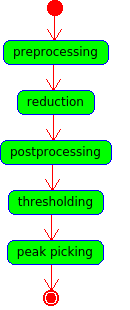
\includegraphics{./onsetActivityDiagram.png}
 % onsetActivityDiagram.png: 322x477 pixel, 96dpi, 8.52x12.62 cm, bb=0 0 241 358
   \end{center}
   \caption{Diagramma di attivit\`a di un generico algoritmo di beat detection}
   \label{onsetActivityDiagram}
 \end{wrapfigure}
    La riduzione \`e il processo di trasformare il segnale audio in un segnale con una frequenza di campionamento molto piu' ridotta e che manifesta in modo piu' evidente la posizione degli onset. Questo \`e il cuore degli algoritmi di onset detection. Chiamiamo l'output di questa fase anche detection function. Classifichiamo i metodi di riduzione in due categorie: metodi basati su caratteristiche esplicite del segnale e metodi basati su modelli probabilistici. 
    \paragraph{Metodi basati su caratterische esplicite del segnale.}
    Le caratteristiche esplicite di un segnale possono rientrare nelle categorie: temporali, spettrali, spettrali di fase e spettrotemporali. 
    \paragraph{Caratterische temporali.}
	Nel dominio del tempo del segnale si nota spesso che una occorrenza di un onset di solito \`e accompagnata da un aumento dell'ampiezza del segnale. Alcuni metodi di onset detection si avvantaggiano di questa propriet\`a e creano una detection function che segue l'envelope del segnale. Questi metodi danno risultati soddisfacenti nei casi in cui c'\`e un onset molto forte rispetto al sottofondo. 
%     \paragraph{caratterische spettrali} DA FARE
    \paragraph{Metodi basati su modelli probabilistici.}
      I metodi statici per l'onset detection sono basati sull'assunto che il segnale pu\`o essere descritto da qualche modello di probabilit\`a. Quindi si pu\`o costruire un sistema che fa inferenza probabilistica riguardo i tempi probabili di cambiamenti improvvisi nel segnale in base alle osservazioni disponibili. Il successo di questo approccio dipende dalla somiglianza tra la distribuzione di probabilit\`a descritta dal modello e la distribuzione reale dei dati e si pu\`o quantificare usando modelli di selezione Bayesiani. Ci sono vari metodi di questo tipo.

% background. A variation on this is to follow the local energy,
% rather than the amplitude, by squaring, instead of rectifying,
% each sample
% (2)
% Despite the smoothing, this reduced signal in its raw form is
% not usually suitable for reliable onset detection by peak picking.
% A further refinement, included in a number of standard onset
% detection algorithms, is to work with the time derivative of the
% energy (or rather the first difference for discrete-time signals) so
% that sudden rises in energy are transformed into narrow peaks in
% the derivative. The energy and its derivative are commonly used
% in combination with preprocessing, both with filter-banks [3]
% and transient/steady-state separation [9], [19].
% Another refinement takes its cue from psychoacoustics: em-
% pirical evidence [20] indicates that loudness is perceived loga-
% rithmically. This means that changes in loudness are judged rel-
% ative to the overall loudness, since, for a continuous time signal,
% . Hence, computing the first-dif-
% roughly simulates the ears perception of
% ference of
% loudness. An application of this technique to multiple bands [5]
% showed a significant reduction in the tendency for amplitude
% modulation to cause the detection of spurious onsets.
% 

%   \subsection{peak picking}
%     Se la detection function \`e stata progettata bene, allora gli onset danno luogo a caratterische ben localizzate e facilmente identificabili nella detection function. Di solito queste caratterische sono massimi locali o \emph{peak}, generalmente soggetti a qualche livello di variabilit\`a in forma e dimensione, e mascherati da rumore. Dunque un algoritmo robusto di scelta dei picchi ha bisogno di stimare il tempo di onset degli eventi nell'analisi del segnale. Dividiamo il processo di scelta dei picchi in tre fasi: 
  \subsection{Postprocessing}
	Questa fase \`e opzionale e serve per facilitare le fasi successive attraverso l'aumento dell'uniformit\`a e dela consistenza di alcuni aspetti della detection function che vengono trasformati in massimi locali isolati e facili da trovare. In questa fase possiamo trovare ad esempio: algoritmi di riduzione del rumore e algoritmi di selezione di parametri utili al calcolo del thresholding nelle fasi successive.

  \subsection{Thresholding}
	Ci possono essere dei picchi nella detection function che non sono correlati ad un onset di interesse. Quindi \`e necessario definire un threshold che separi in modo efficacie i picchi che corrispondono ad un evento di interesse e quelli che non vi corrispondono. In questa fase un onset che corrisponde ad un evento di interesse \`e definito come un picco nel quale la detection function supera una certa soglia. Ci sono due approcci principali alla scelta della soglia:
	\begin{description}
	  \item[Thresholding fisso.]
	    La soglia in questione non varia nel corso della vita dell'algoritmo.
	  \item[Thresholding adattativo.]
	    La soglia in questione varia ed \`e di solito una certa funzione della detection function. Ad esempio:
	    \begin{description}
	      \item[Linear smoothing.]
		La soglia \`e una combinazione lineare degli elementi all'interno della finestra corrente della detection function.
	      \item[Non linear smoothing.]
		La soglia \`e una combinazione non lineare degli elementi all'interno della finestra corrente della detection function. Ad esempio una combinazione dei quadrati.
	      \item[Percentiles smoothing.]
		I metodi precedenti hanno lo svantaggio che quando ci sono dei picchi relativamente grandi seguiti da picchi piccoli, questi ultimi vengono nascosti. Per evitare questo problema si posso usare metodi basati sui percentili ad esempio la mediana. 
	    \end{description}
	\end{description}
  \subsection{Peak picking}
    Nella fase di scelta dei picchi si devono solamente identificare i massimi locali al di sopra del threshold. 


% For a review of a number of peak-picking algorithms for audio signals, see \cite{TFTAAOMA}. 


% For our experiments the detection functions were first nor-
% malized by subtracting the mean and dividing by the maximum
% absolute deviation, and then low-pass filtered. An adaptive
% threshold, calculated using a moving-median filter [(21)], was
% then subtracted from the normalized detection function. Finally,
% every local maximum above zero was counted as an onset. Both
% the filter and the thresholding parameters (cutoff frequency,
% , and ) were hand-tuned based on experimenting, thus
% resulting in a separate parameter set for each detection function.
% Values for the cutoff frequency are selected according to the in-
% herent characteristics of each detection method, as discussed in section IIIC
% is set to the longest time interval on which the
% global dynamics are not expected to evolve (around 100 ms);
% while is set to 1, as it is not critical for the detection. However,
% experiments show sensitivity to variations of , such that error
% rates can be minimized by changing it between different types
% of music signals (e.g., pitched percussive, nonpercussive, etc).


 

% I metodi temporali nella fase di riduzione sono semplici e computazionalmente efficienti. Il loro funzionamento dipende dall'esistenza di aumenti chiaramente identificabili nell'ampiezza del segnale. La robustezza dei metodi basati sull'ampiezza diminuisce in presenza di modulazioni di ampiezza e di sovrapposizione di energie prodotte da suoni simultanei. Questo rimane vero anche se si divide il segnale in bande. 
% Per suoni non banali, gli schemi di onset detection beneficiano dell'uso di rappresentazioni piu' ricche del segnale(frequenza rispetto al tempo).  
% 
% The commonly used HFC [22, eq. (4)] is an example of a spectral weighting method. It is successful at emphasizing the percussiveness of the signal [cf. Figs. 5 and 6], but less robust at detecting the onsets of low-pitched and nonpercussive events [cf. Fig. 4], where energy changes are at low frequencies and hence de-emphasized by the weighting. 
% 
% In some signals, even broadband onsets are susceptible to masking by continuous high-frequency content such as that due to open cymbals in a pop recording. This problem can be overcome by using temporal difference methods such as the norm of the rectified spectral difference [[6, eq. (5)], as these can respond to changes in the distribution of spectral energy, as well as the total, in any part of the spectrum. However, the difference calculation relies solely on magnitude information, thus neglecting the detection of events without a strong energy increase: e.g., low notes, transitions between harmonically related notes or onsets played by
% bowed instruments (cf. Fig. 4). 
% 
% I metodi basati sulla fase, such as the spread of the distribution
% of phase deviations in (9) (see [25]), are designed to compensate for such shortcomings. They are successful at detecting low and high-frequency tonal changes regardless of their intensity. The approach suffers from variations introduced by the phases of noisy low-energy components, and from phase distortions common to complex commercial music recordings (e.g., audio effects, post-production treatments—cf. Fig. 6). The wavelet regularity modulus [29] in (12), is an example of an approach using an alternative time-scale representation that can be used to precisely localize events down to a theoretical resolution of as little as two samples of the original signal, which for typical audio sampling rates is considerably better than the ears resolution in time. The price of this is a much less smooth detec- tion function (cf. all figures), therefore emphasizing the need for post-processing to remove spurious peaks. The method provides an interesting alternative to other feature-based methods, but with an 
% increase in algorithmic complexity. Approaches based on probabilistic models provide a more general theoretical view of the analysis of onsets. As shown in Section III-B.2, previous reduction methods can be explained within the context of measuring surprise relative to a proba- bilistic model, while new methods can be proposed and evaluated by studying refinements or alternatives to existing models. An example is the surprise-based method using ICA to model the conditional probability of a short segment of the signal, calculated in (17) as the difference between two negative log-likelihoods [35]. If the model is adequate (i.e., the assumptions be- hind the model are accurate and the parameters well-fitted), then robust detection functions for a wide range of signals can be pro- duced. Examples are at the bottom of Figs. 4–6. However, for adaptive statistical models such as ICA, these advantages accrue only after a potentially expensive and time-consuming training process during which the parameters of the 
% model are fitted to a given training set.
% 






% \chapter{Online onset detection model}
% \cite{TFTAAOMA}:




\section{Clustering}
\label{clustering}
Il clustering \`e il processo di trovare informazioni strutturali all'interno di un insieme di dati. 
I meccanismi di clustering separano e organizzano dati non etichettati in vari gruppi o cluster, ognuno dei quali contiene dati che sono simili tra loro. 
Un buon algoritmo di clustering produce cluster nel quale la somiglianza intracluster, cio\`e tra gli elementi di un cluster, \`e alta mentre la somiglianza intercluster, cio\`e tra elementi di cluster diversi, \`e bassa. 
Per una discussione approfondita sul clustering si rimanda a \cite{PatternRecognition}.

Se vogliamo essere piu' formali possiamo dire che un $m-clustering$ di un insieme di dati $X$ rispetto ad una distanza o misura di dissimilarit\`a $d:P(X)\rightarrow \mathbb{R}$ e ad una soglia $t$ \`e $C_{1}, \cdots, C_{n}$ tale che:
\begin{description}
  \item[partizione]
    $C_{1}, \cdots, C_{n}$ \`e una partizione di $X$ cio\`e: ogni $C_{i}$ \`e un sottoinsieme di $X$; i $C_{i}$ sono a due a due disgiunti; l'unione dei $C_{i}$ d\`a $X$
  \item[intersimilarit\`a]
    per ogni $i$: $d(C_{i})<t$
\end{description}



  
Di seguito descriveremo alcuni tipi di algoritmi di clustering. 
Ci sono due tipi principali di algoritmi di clustering a seconda dei parametri di input. 
Una categoria di algoritmi prende in input il numero di cluster, oltre che gli elementi di input e la funzione di dissimilarit\`a, e restituisce un clustering dei dati. 
Una seconda categoria di algoritmi prende in input un valore di soglia e restituisce un clustering.
\paragraph{Clustering sequenziale.}
  Questi algoritmi leggono gli elementi di input uno per volta in sequenza. 
  In questo tipo di algoritmi non conosciamo a priori il numero di cluster presenti nell'input. 
  Invece prendono in input una soglia $\theta$ e il massimo numero di cluster permessi $q$. 
  L'idea alla base di questi algoritmi \`e che quando viene letto un elemento, questo viene o assegnato ad un cluster esistente o ad un nuovo cluster a seconda della distanza tra l'elemento e i cluster esistenti. 
  Uno schema generale per implementare un algoritmo di clustering sequenziale \`e dati in figura \ref{clusteringSequenzialeAlgoritmo}.

\incmargin{1em}
\restylealgo{boxed}\linesnumbered
\begin{algorithm}
  \dontprintsemicolon
  \SetVline
  % \SetNoline
%   \SetKwData{b}{b}
%   \SetKwData{This}{this}
%   \SetKwData{Up}{up}
  \SetKwFunction{getAverageLocalEnergy}{getAverageLocalEnergy}
  \SetKwFunction{getInstantSoundEnergy}{getInstantSoundEnergy}
  \SetKwFunction{Write}{write}
  \SetKwFunction{Init}{init}
  \SetKwFunction{Clear}{clear}
  \SetKwFunction{Add}{add}
  \SetKwFunction{DDDD}{distance}
  \SetKwInOut{Input}{input}
  \SetKwInOut{Output}{output}
  \caption{Sequential clustering algorithm}
    \Input{A sequence of data $x_{1}, \cdots, x_{n}$}
    \Output{A clustering of the data $C_{1}, \cdots, C_{m}$}
    \BlankLine
    $m\leftarrow 1$\;
    $C_{m}\leftarrow \{x_{1}\}$\;
    \For{$i\leftarrow 2$ \KwTo $n$}{
      find $k$ such that the distance between $x_{i}$ and $C_{k}$ is minimum\;
       \eIf{$\DDDD(x_{i}, C_{k}) > $ threshold}{
 	increments $m$\;
 	$C_{m}\leftarrow \{x_{i}\}$\;
       }{
 	$C_{m}\leftarrow C_{m}\cup \{x_{i}\}$\;
       }
  }
\label{clusteringSequenzialeAlgoritmo}
\end{algorithm}
\decmargin{1em}

Un algoritmo di clustering sequenziale si dice \emph{a cluster sequenziali} se produce cluster sequenziali e cio\`e \`e tale che ad ogni iterazione: o si aggiunge l'elemento corrente nello stesso cluster dell'iterazione precedente, o si aggiunge l'elemento in un nuovo cluster.

Se non si conosce in anticipo neanche il valore di soglia allora si pu\`o stimare il numero di cluster che ci sono nell'input usando l'algoritmo \ref{determinareClusterN}. 

\incmargin{1em}
\restylealgo{boxed}\linesnumbered
\begin{algorithm}
  \dontprintsemicolon
  \SetVline
  % \SetNoline
%   \SetKwData{b}{b}
%   \SetKwData{This}{this}
%   \SetKwData{Up}{up}
  \SetKwFunction{getAverageLocalEnergy}{getAverageLocalEnergy}
  \SetKwFunction{getInstantSoundEnergy}{getInstantSoundEnergy}
  \SetKwFunction{Write}{write}
  \SetKwFunction{Init}{init}
  \SetKwFunction{Clear}{clear}
  \SetKwFunction{Add}{add}
  \SetKwFunction{DDDD}{distance}
  \SetKwInOut{Input}{input}
  \SetKwInOut{Output}{output}
  \caption{Algoritmo di stima del numero dei cluster. Usato nella sezione \ref{clusteringMetodologia}}
    \Input{A sequence of data $x_{1}, \cdots, x_{n}$}
    \Output{An estimation of the number of clusters}
    \BlankLine
    \For{threshold $\leftarrow$ a \KwTo b step c}{
      run clustering algorithm with current threshold\;
      store the number of clusters obtained\;
    }
    \Return the most frequent number of clusters\;
\label{determinareClusterN}
\end{algorithm}
\decmargin{1em}



\paragraph{Clustering gerarchico.}
Il clustering gerarchico \`e un approccio di clustering che mira a costruire una gerarchia di cluster. 
Le strategie per il clustering gerarchico sono tipicamente di due tipi:
\begin{description}
  \item[Agglomerativo] 
    questo tipo di algoritmo produce una sequenza di clustering che hanno numero di cluster decrescente. 
  \item[Divisivo]
    questo tipo di algoritmo produce una sequenza di clustering che hanno numero di cluster crescente. 
    Ad ogni iterazione un algoritmo di questo tipo prende i cluster risultati dall'iterazione precedente e li divide.
\end{description}


\paragraph{Algoritmi di clustering basati su una funzione di ottimizzazione del costo.}
In questi algoritmi il numero di cluster \`e fisso. 
Si cerca di assegnare gli elementi di input ai cluster in modo da ottimizzare il valore di una funzione di costo. 



% Provare: 
%   mantenere il massimo e il minimo dell'energia di una finestra di 10ms
%   se l'energia di una finestra \`e maggiore dell'ottanta per cento del massimo allora \`e un beat, se \`e minore del 120 per cento  del minimo allora \`e silenzio
%   il respiro \`e beat seguito da non beat



% provare: 
% vari thread di esecuzione, ognuno un k clustering online sequenziale, k va da 1 a 10, quello che raggiunge una maggiore qualit\`a di clustering \`e l'algoritmo corretto
\section{Reti neurali}
\label{retineurali}
Le \emph{reti neurali artificiali} sono modelli matematici e computazionali della corteccia cerebrale. 
Gli elementi di base di una rete neurale artificiale sono:
\begin{description}
  \item[neuroni artificiali o unita']
%     neuroni artificiali o \emph{unita'} 
  \item[collegamenti]
    I neuroni artificiali sono connessi attraverso \emph{collegamenti}. 
    Ogni collegamento ha un \emph{peso} numerico, in particolare il collegamento tra l'unita' $i$ e l'unita' $j$ ha peso $w_{i,j}$. 
\end{description}
Una certa unita' $i$ pu\`o inviare un \emph{segnale} o \emph{attivazione} $a_{i}$ su tutti i suoi collegamenti. 
Il peso di un collegamento determina la forza e il segno del segnale. 
Assumiamo l'esistenza di una certa unita' di input che manda il segnale $a_{0}$. 
Ogni unita' si comporta nel modo seguente:
\begin{enumerate}
  \item 
    calcola la somma pesata dei suoi input
    \begin{center}
      $in_{j} = \sum\limits_{i=0}^n w_{i,j} a_{i}$
    \end{center}
  \item
    calcola il proprio output in base al valore calcolato al punto precedente e ad una \emph{funzione di attivazione} $g$: 
    \begin{center}    
      $a_{j}=g(in_{j})$
    \end{center}    
\end{enumerate}
La funzione di attivazione di solito \`e una funzione del tipo:
\begin{center}
  \begin{tabular}{lll}
      $g(x)= \left\{ 
	  \begin{array}{ll}
	      0
	    &
	      if\; x< 0
	    \\
	      1
	    &
	      if\; x> 0
	  \end{array}
      \right.$
    &
      o
    &
      $g(x)= \frac{1}{1+e^{-x}}$
  \end{tabular}
\end{center}

Ci sono due tipi di reti neurali:
\begin{description}
  \item[feed forward]
    I collegamenti tra unita' sono unidirezionali. 
    In questo caso la rete neurale \`e un grafo diretto aciclico. 
    Una rete neurale di tipo feed forward rappresenta una funzione dei suoi input nel senso che non ha uno stato interno o memoria. 
    Una rete feed forward \`e di solito divisa in \emph{layers} o livelli. 
    Ogni livello \`e un insieme di unita', ogni unita' riceve input solo da unita' del livello immediatamente precedente. 
    Una rete con un solo livello si dice anche \emph{single-layer} o \emph{monolivello}.
  \item[recurrent network]
    Ci possono essere dei cicli nei collegamenti. 
    Una rete di questo tipo rappresenta un sistema dinamico che pu\`o anche oscillare o avere un comportamento caotico. 
    Inoltre la riposta di una recurrent network dipende dallo stato iniziale della rete e dall'input quindi questo tipo di rete pu\`o supportare una memoria a breve termine.
\end{description}


\section{Dimensione frattale}
\label{frattale}
In geometria frattale la dimensione frattale \`e una quantit\`a statistica che da una indicazione di quanto completo appare un frattale per riempire lo spazio. 
La dimensione frattale inoltre \`e una misura della complessit\`a di un insieme di dati. 
Viene usata per analizzare segnali in un vasto numero di ricerche scientifiche. 
Una propriet\`a della dimensione frattale \`e che \`e indipendente dal contenuto di energia nel segnale ma \`e dipendente dalle frequenze. 
Ci sono molti modi di definire matematicamente la dimensione frattale ad esempio quello illustrato in \cite{RSDUVFD}:
\[
  D_{\sigma} = \displaystyle\lim_{\delta t \rightarrow 0} \frac{\log(Var(\delta S, \delta t))}{2 \cdot \log(\delta t)}
\]
In questa formula: $\delta t$ \`e il valore assoluto di una variazione temporale $|t_{2}-t_{1}|$ mentre $\delta S$ \`e la variazione del segnale nel tempo $S(t_{2})-S(t_{1})$.



 
\section{Catene di triple Markoviane}
\label{markov}
\subsection{Nozioni di base di probabilit\`a}

\paragraph{Evento. Spazio Campionario.}Dato un esperimento casuale, definiamo un evento elementare $\omega$ come uno dei possibili esiti dell'esperimento stesso. Definiamo un evento come un qualsiasi insieme di eventi elementari. Definiamo lo spazio campionario come l'insieme di tutti gli eventi elementari. Uno spazio campionario si indica di solito con il nome $\Omega$.

\paragraph{$\sigma-$algebra}
Dato un insieme $\Omega$, si definisce $\sigma-$algebra su $\Omega$ una famiglia $F$ di sottoinsiemi di $\Omega$ tale che:
\begin{itemize}
  \item 
    $\Omega$ appartiene ad $F$.
  \item
    L'insieme $F$ \`e chiuso rispetto a complementare.
  \item
    L'insieme $F$ \`e chiuso rispetto ad unione numerabile.
\end{itemize}.

\paragraph{Spazio misurabile. Insiemi misurabili.}
Uno spazio misurabile \`e una coppia $(\Omega, F)$ tale che $F$ \`e una $\sigma-$algebra su $\Omega$. Gli elementi di $F$ sono detti insiemi misurabili in $\Omega$.

\paragraph{Topologia. Spazio topologico.}
Dato un insieme $X$, una topologia su $X$ \`e un insieme $T$ di sottoinsiemi di $X$ tale che:
\begin{itemize}
  \item 
    L'insieme vuoto e $X$ appartengono a $T$.
  \item
    L'unione di una quantit\`a arbitraria di insiemi appartenenti a $T$ appartiene a $T$.
  \item
    L'intersezione di un numero finito di insiemi appartenenti a $T$ appartiene a $T$.
\end{itemize}
Uno spazio topologico \`e una coppia $(X, T)$, dove $X$ \`e un insieme e $T$ \`e una topologia su $X$. In uno spazio topologico gli insiemi che costituiscono $T$ si dicono aperti in $X$.

\paragraph{Funzione misurabile.}
Sia $(X,F)$ uno spazio misurabile e $(Y,T)$ uno spazio topologico. Una funzione $f:X\rightarrow Y$ viene detta misurabile se la controimmagine di ogni elemento di $T$ \`e in $F$.


\paragraph{Variabile casuale o aleatoria.}
Sia dato uno spazio campionario $\Omega$ su cui \`e definita una misura di probabilit\`a $\nu$, una variabile casuale \`e una funzione misurabile dallo spazio campionario a uno spazio misurabile. 


\paragraph{Processo stocastico.}
Si definisce processo stocastico una famiglia di variabili aleatorie  
\[
  \{X(T)|\; t\in T\subseteq \mathbf{R}^{+}\}
\]
dipendenti dal tempo, definite su un unico spazio campione $\Omega$ finito e che assumono valori in un insieme definito spazio degli stati del processo. Un processo stocastico \`e quindi un insieme di funzioni che evolvono nel tempo, ognuna delle quali \`e associata ad un determinato elemento dello spazio campione, cos\`i che il risultato di un esperimento casuale corrisponde di fatto all'estrazione di una di queste funzioni.
Un processo stocastico discreto \`e un processo stocastico nel quale $T$ \`e un sottoinsieme dei numeri naturali.


\subsection{Processo di Markov}
Un processo stocastico markoviano o processo di Markov \`e un processo stocastico nel quale la probabilit\`a di transizione che determina il passaggio ad uno stato di sistema dipende unicamente dallo stato di sistema immediatamente precedente (propriet\`a di Markov) e non dal come si \`e giunti a tale stato. Formalmente questo pu\`o essere scritto come
\[P(X_{n+1}\leq x_{n+1} |_{i=1}^{n} X_{i}\leq x_{i}) = P(X_{n+1}\leq x_{n+1} | X_{n}\leq x_{n})\]
Questa \`e detta propriet\`a di Markov, o condizione di assenza di memoria.

\subsection{Catena di Markov}
Una catena di Markov \`e un processo di Markov con spazio degli stati discreto, quindi si tratta di un processo stocastico che assume valori in uno spazio discreto e che gode della propriet\`a di Markov. L'insieme  di spazio degli stati pu\`o essere finito o infinito (numerabile). Nel primo caso si parla di catena di Markov a stati finiti. Una catena di Markov pu\`o essere tempo-continua o tempo-discreta, in base all'insieme di appartenenza della variabile tempo (continuo o discreto).
Formalmente, una catena di Markov \`e una sequenza di variabili aleatorie $X_{1}, X_{2}, \cdots, $ che soddisfa la condizione di Markov.


\subsection{Modelli nascosti di Markov}

In un modello nascosto di Markov abbiamo due processi stocastici: il processo di interesse inosservabile $X=(X_{s})_{s\in S}$ e il processo osservabile $Y=(Y_{s})_{s\in S}$. Un modello nascosto di Markov \`e $(X, Y, T, E, \pi)$ tale che:
\begin{description}
  \item
    $T:X\times X\rightarrow [0;1]$ \`e la probabilit\`a di transizione. In particolare 
    \[	
      p(X_{t+1}=x_{i}| X_{t}=x_{j})=T(x_{i},x_{j})
    \] 
    \`e la probabilit\`a che il processo nascosto passi dallo stato $x_{i}$ allo stato $x_{j}$.
  \item
    $E:X\times Y \rightarrow [0;1]$ \`e la probabilit\`a condizionata di $X$ rispetto ad $Y$. Cio\`e se osserviamo un certo valore $y$ per il processo osservabile $Y$ allora $E$ ci dice qual'\`e la probabilit\`a che il processo nascosto assuma certi valori.
  \item
    $\pi:X\rightarrow [0;1]$ \`e la probabilit\`a iniziale che il processo nascosto si trovi in un certo stato.
\end{description}






\subsection{Catena di coppie markoviane}


Supponiamo che $X = (X_{1}, \cdots, X_{n})$ e $Y = (Y_{1}, \cdots, Y_{1})$ siano due processi stocastici, nei quali ogni $X_{i}$ ha valori in un insieme finito $\Omega=\{\omega_{1}, \cdots, \omega_{n}\}$ e ogni $Y_{i}$ ha valori reali. Sia $Z = (Z_{1}, \cdots, Z_{n})$ il processo stocastico delle coppie di $X,Y$, cio\`e $Z_{i}=(X_{i}, Y_{i})$. 
I processi $X$ e $Y$ sono una catena di coppie markoviane se $Z$ \`e un processo di Markov cio\`e quando 
\[
  p(z)=p(z_{1}) p(z_{2}|z_{1}) \cdots p(z_{n}|z_{n-1})
\]



\subsection{Catena di triple markoviane}

Le catene di triple markoviane sono una estensione delle catene di coppie di Markov nelle quali la distribuzione di probabilit\`a di $(X,Y)$ \`e una distribuzione di probabilit\`a marginale di una catena di Markov $(X,U,Y)$.
Anche nelle catene di triple markoviane cerchiamo $X$ a partire da $Y$, il processo $S$ serve solo come aiuto al calcolo. 
Sia $S=N$ l'insieme dei numeri naturali senza lo zero e siano $X=(X_{n})_{n\in N}$, $Y=(Y_{n})_{n\in N}$, $U=(U_{n})_{n\in N}$ tre processi, nei quali le variabili $X_{i}$ assumono valori in uno spazio campionario $\Omega=\{\omega_{1}, \cdots, \omega_{k}\}$, le variabili $Y_{i}$ sono a valori reali e le variabili $U_{i}$ assumono  
valori nell'insieme $\Lambda = \{\lambda_{1}, \cdots, \lambda_{m}\}$.
Con lo scopo di semplificare la notazione, poniamo $T_{n}=(X_{n}, U_{n}, Y_{m})$, $Z_{n}=(X_{n}, Y_{n})$ e $V_{n}=(X_{n}, U_{n})$ e chiamiamo $T,Z$ e $V$ i processi corrispondenti.
Diremo che $Z$ \`e una catena di triple di Markov se esiste un processo $U$ nel quale $T$ \`e una catena di Markov.
In questo caso allora $(V,Y)$ \`e una catena di Coppie di Markov. Possiamo scrivere la distribuzione di probabilit\`a di $(V_{i}, Y)$ come 
\[
  p(v_{i}, y)=\alpha^{i}(v_{i}) \beta^{i}(v_{i})
\]
con $\alpha^{i}(v_{i})$ e $\beta^{i}(v_{i})$ definite rispettivamente come 
\[
  \begin{array}{ll}
      \alpha^{i}(v_{i})=p(y_{1}, \cdots, y_{i-1}, y_{i}, v_{i})
    &
      \beta^{i}(v_{i})=p(y_{i+1}, \cdots, y_{n}, v_{i}, y_{i})
  \end{array}
\]


